%%%%%%%%%%%%%%%%%%%%%%%%%%%%%%%%%%%%%%%%%
% Short Sectioned Assignment
% LaTeX Template
% Version 1.0 (5/5/12)
%
% This template has been downloaded from:
% http://www.LaTeXTemplates.com
%
% Original author:
% Frits Wenneker (http://www.howtotex.com)
%
% License:
% CC BY-NC-SA 3.0 (http://creativecommons.org/licenses/by-nc-sa/3.0/)
%
%%%%%%%%%%%%%%%%%%%%%%%%%%%%%%%%%%%%%%%%%

%----------------------------------------------------------------------------------------
%	PACKAGES AND OTHER DOCUMENT CONFIGURATIONS
%----------------------------------------------------------------------------------------

\documentclass[paper=a4, fontsize=11pt]{scrartcl} % A4 paper and 11pt font size

\usepackage{algorithm2e}
\usepackage{algorithm}
\usepackage{algpseudocode}
\usepackage{graphicx}
\usepackage{float}
\graphicspath{ {images/} }
\usepackage{subcaption}
\usepackage[export]{adjustbox}
\usepackage[T1]{fontenc} % Use 8-bit encoding that has 256 glyphs
\usepackage[english]{babel} % English language/hyphenation
\usepackage{amsmath,amsfonts,amsthm} % Math packages

\usepackage{lipsum} % Used for inserting dummy 'Lorem ipsum' text into the template

\usepackage{sectsty} % Allows customizing section commands
\allsectionsfont{\centering \normalfont\scshape} % Make all sections centered, the default font and small caps

\usepackage{fancyhdr} % Custom headers and footers
\pagestyle{fancyplain} % Makes all pages in the document conform to the custom headers and footers
\fancyhead{} % No page header - if you want one, create it in the same way as the footers below
k\fancyfoot[L]{} % Empty left footer
\fancyfoot[C]{} % Empty center footer
\fancyfoot[R]{\thepage} % Page numbering for right footer
\renewcommand{\headrulewidth}{0pt} % Remove header underlines
\renewcommand{\footrulewidth}{0pt} % Remove footer underlines
\setlength{\headheight}{13.6pt} % Customize the height of the header

\numberwithin{equation}{section} % Number equations within sections (i.e. 1.1, 1.2, 2.1, 2.2 instead of 1, 2, 3, 4)
\numberwithin{figure}{section} % Number figures within sections (i.e. 1.1, 1.2, 2.1, 2.2 instead of 1, 2, 3, 4)
\numberwithin{table}{section} % Number tables within sections (i.e. 1.1, 1.2, 2.1, 2.2 instead of 1, 2, 3, 4)

\setlength\parindent{0pt} % Removes all indentation from paragraphs - comment this line for an assignment with lots of text

%----------------------------------------------------------------------------------------
%	TITLE SECTION
%----------------------------------------------------------------------------------------

\newcommand{\horrule}[1]{\rule{\linewidth}{#1}} % Create horizontal rule command with 1 argument of height

\title{	
\normalfont \normalsize 
\textsc{CS 2810, Advanced Programming Lab} \\ [25pt] % Your university, school and/or department name(s)
\horrule{0.5pt} \\[0.4cm] % Thin top horizontal rule
\huge Visualization of Dinic Algorithm\\ % The assignment title
\horrule{2pt} \\[0.5cm] % Thick bottom horizontal rule
}

\author{Rahul Ramesh, Vignesh.M, R.Gowrisankar} % Your name

\date{} % Today's date or a custom date

\begin{document}

\maketitle % Print the title

%----------------------------------------------------------------------------------------
%	PROBLEM 1
%----------------------------------------------------------------------------------------

\section{Problem Definition}

The Dinic Algorithm aims to solve the commonly known maxflow problem. Maximum flow problem tries to find the largest flow from designated source to sink vertices in a flow network. A flow network is given by a directed graph, with the weights representing the maximum possible capacities along that edge.

% two figures side by side
\begin{figure}[h]
\begin{subfigure}{0.5\textwidth}
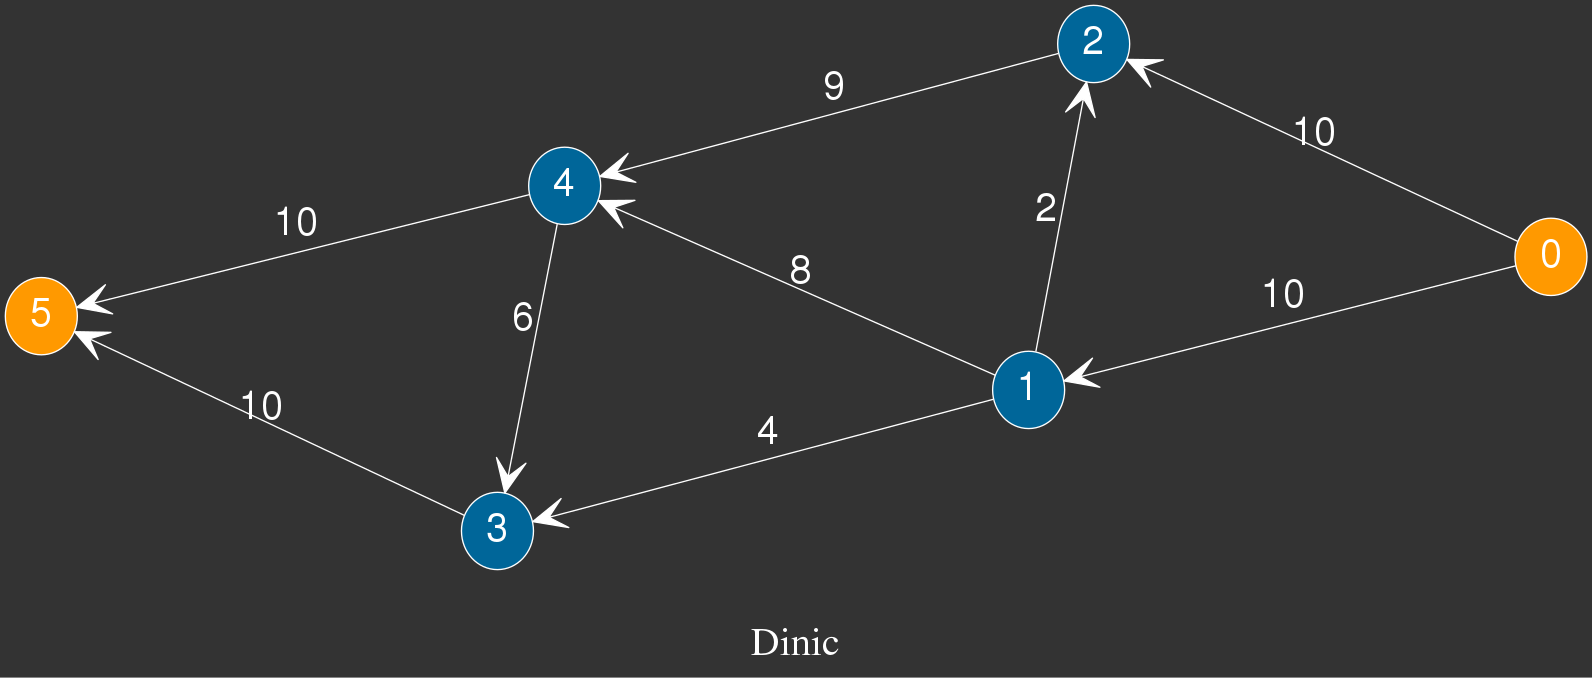
\includegraphics[width=7cm, height=4cm,center]{p1.png}
\caption{Graph showing capacities}
\label{fig:subim1}
\end{subfigure}
\begin{subfigure}{0.5\textwidth}
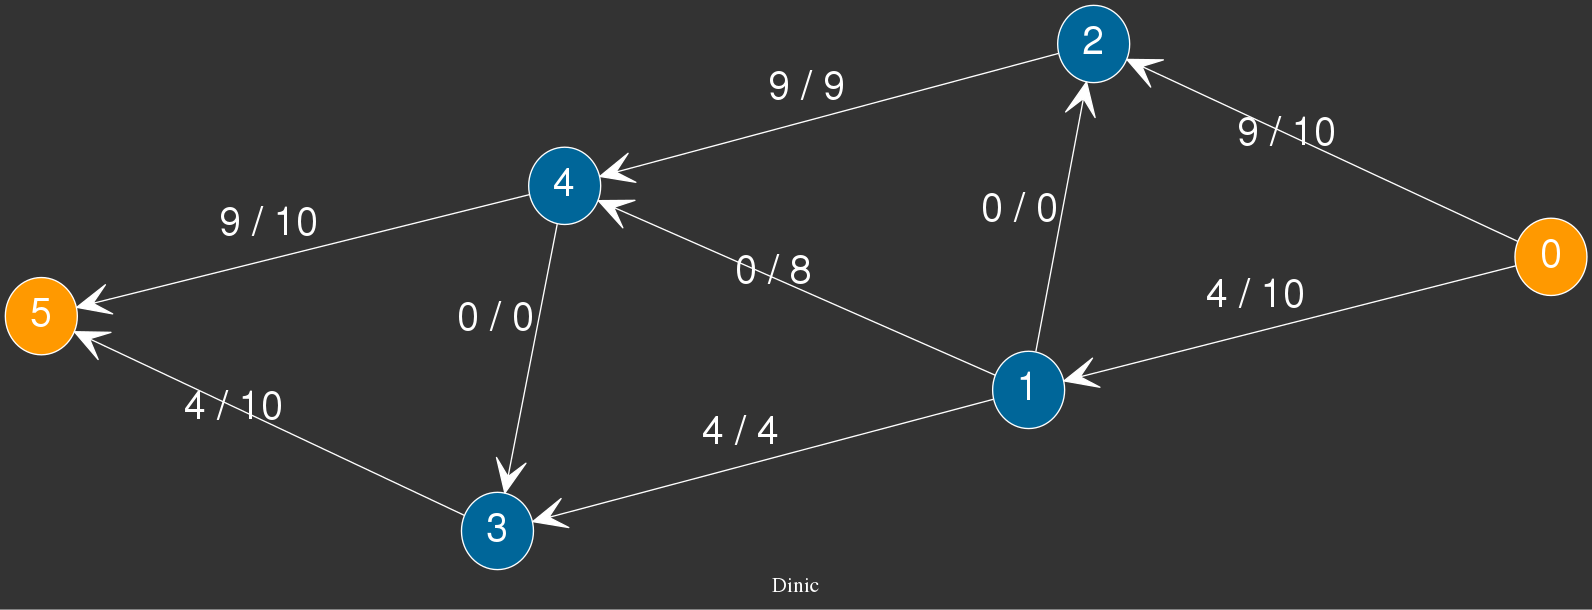
\includegraphics[width=7cm, height=4cm,center]{p4.png}
\caption{Flow-Network}
\label{fig:subim2}
\end{subfigure}

\caption{Example with Source-Sink flow = 13}
\label{fig:image2}
\end{figure}

\begin{figure}[h]
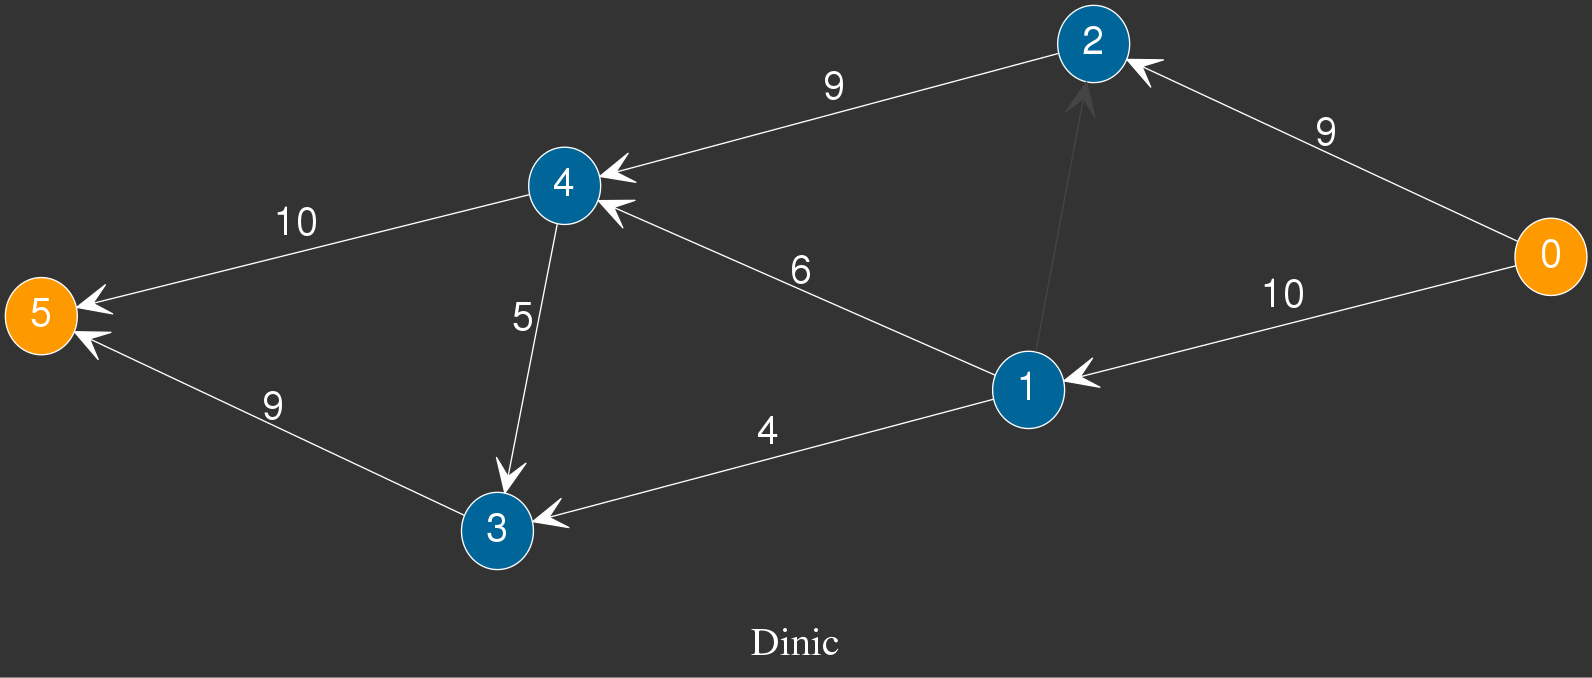
\includegraphics[width=7cm, height=4cm,center]{p2.png}
\caption{Flow-network with Max-flow value after Dinic}
\label{fig:figure2}
\end{figure}

A flow-network is a directed graph where the weights along each edge is sandwiched between zero and the maximum capacity. The value of this weight is known as the flow. The Dinic algorithm gives us a flow-network , such that the flow from the source to the sink is maximised. The same problem can be solved using many algorithms like the Ford-Fulkerson Algorithm, Edmonds-Karp Algorithm Push-Relabel Algorithm or the Dinic Algorithm. We will look at the Dinic Algorithm, and in particular the implementation that runs in $\mathcal{O}(V^2E)$ where V and E are the number of vertices and edges in the graph  Before looking at the algorithm, we will define a few terms like Residual Graph, Level graph and Augmenting Path.


%------------------------------------------------


%----------------------------------------------------------------------------------------
%----------------------------------------------------------------------------------------

\section{Definitions}

%------------------------------------------------

\subsection{Residual Graph}

Consider two vertices V\textsubscript{1} and V\textsubscript{2}. Let the flow from V\textsubscript{1} to V\textsubscript{2} to be F\textsubscript{12} along the edge E\textsubscript{12} and flow from V\textsubscript{2} to V\textsubscript{1} to be F\textsubscript{21} along the edge E\textsubscript{21}. If no edge exists from one vertex to another, then set the flow value to be 0. Also let C\textsubscript{12} and C\textsubscript{21} represent the maximum capacity of edges, E\textsubscript{12} and E\textsubscript{21}.

The Residual graph contains all the vertices present in the original graph. For each pair of vertices V\textsubscript{1}' and V\textsubscript{2}' in the Residual-graph, assign the following:
\begin{align} 
\begin{split}
F_{12}' &= (C_{12} - F_{12} ) + C_{21}\\
F_{21}' &= (C_{21} - F_{21} ) + C_{12}\\
\end{split}					
\end{align}

Residual graph in essence, builds a graph, representing the maximum possible change in flow from V\textsubscript{1} to V\textsubscript{1} or, V\textsubscript{1} to V\textsubscript{1} constrained by the capacities. This graph is used as a tool to increase or decrease flow values along edges, in order to increase the overall source sink-flow. One can discard all edges with zero flow edges in the Residual graph.

\begin{figure}[h]
\begin{subfigure}{0.5\textwidth}
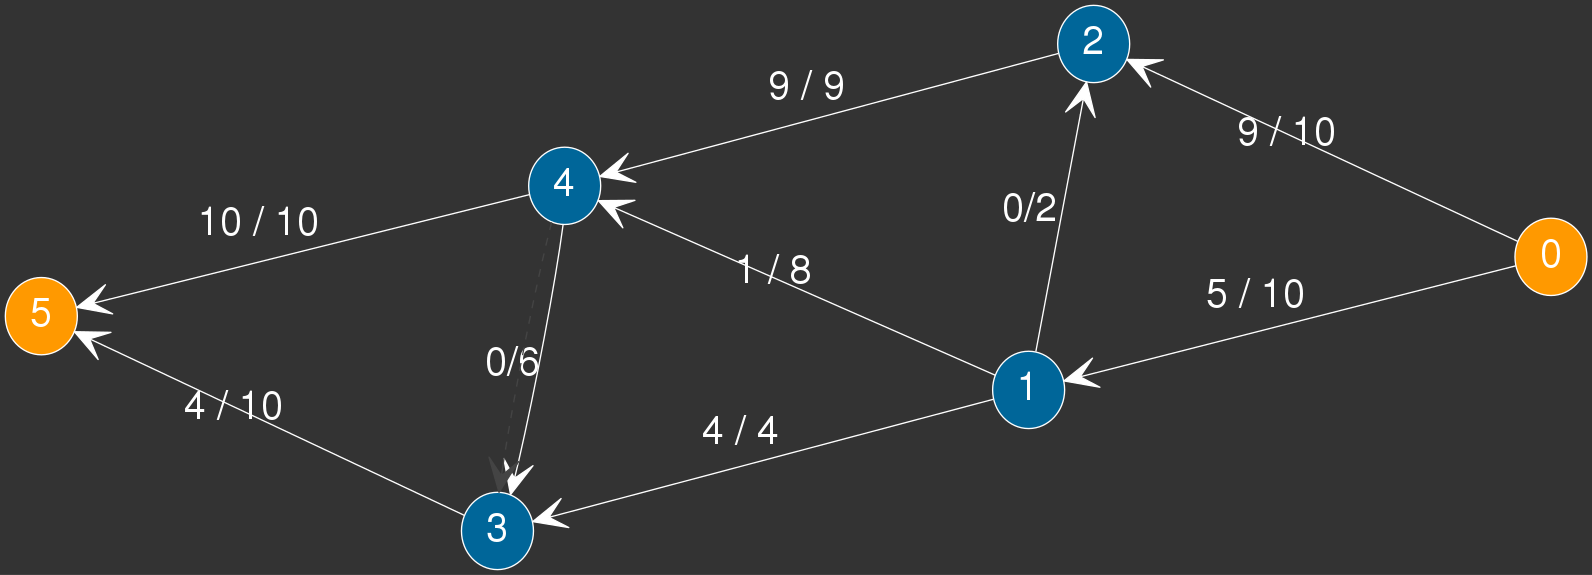
\includegraphics[width=7cm, height=4cm,center]{p6.png}
\caption{Flow-network}
\label{fig:subim1}
\end{subfigure}
\begin{subfigure}{0.5\textwidth}
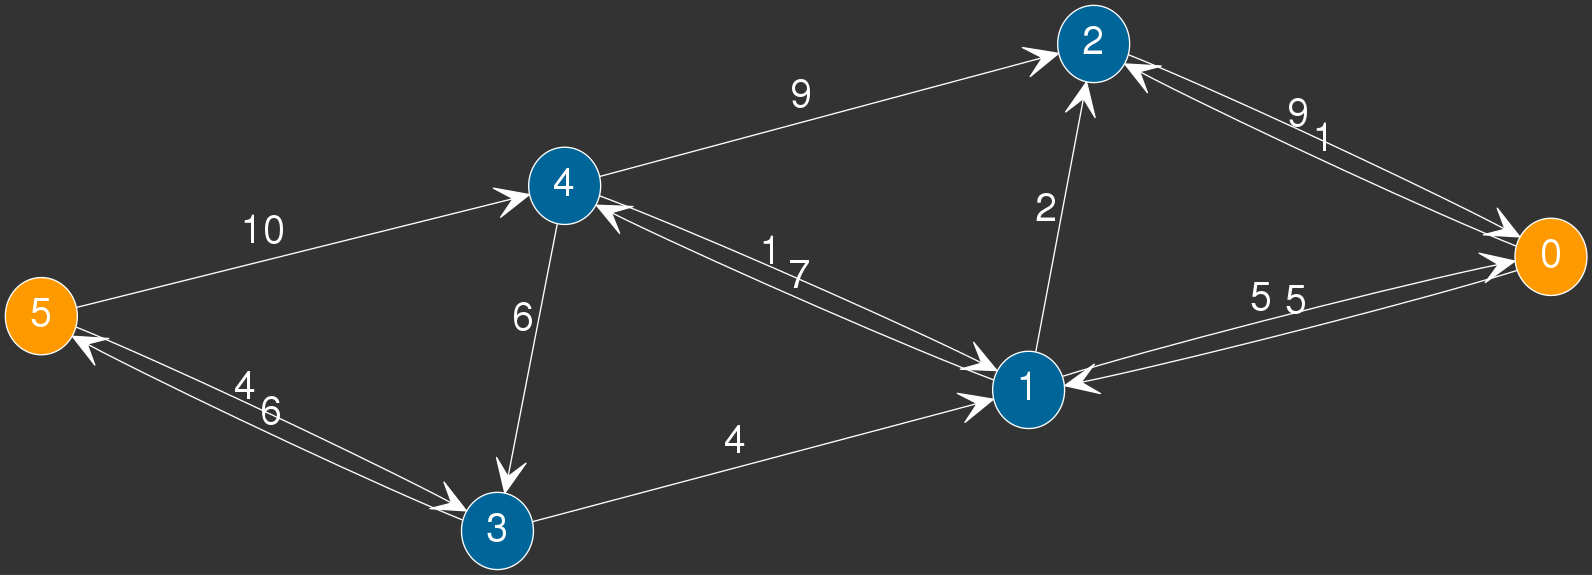
\includegraphics[width=7cm, height=4cm,center]{p5.png}
\caption{Residual graph for Flow-network}
\label{fig:subim2}
\end{subfigure}

\caption{Example for Residual graph}
\label{fig:image2}
\end{figure}

%------------------------------------------------

\subsection{Level Graph}

The Level graph is a sub-graph of the residual graph. Split the vertices in the residual graph into various levels. A vertex is said to belong to level 'i' if the shortest distance from the Source vertex is 'i'. After dividing the vertices into levels, retain only those edges, which go from a level 'i' to level 'i+1'.


\begin{figure}[h]
\begin{subfigure}{0.5\textwidth}
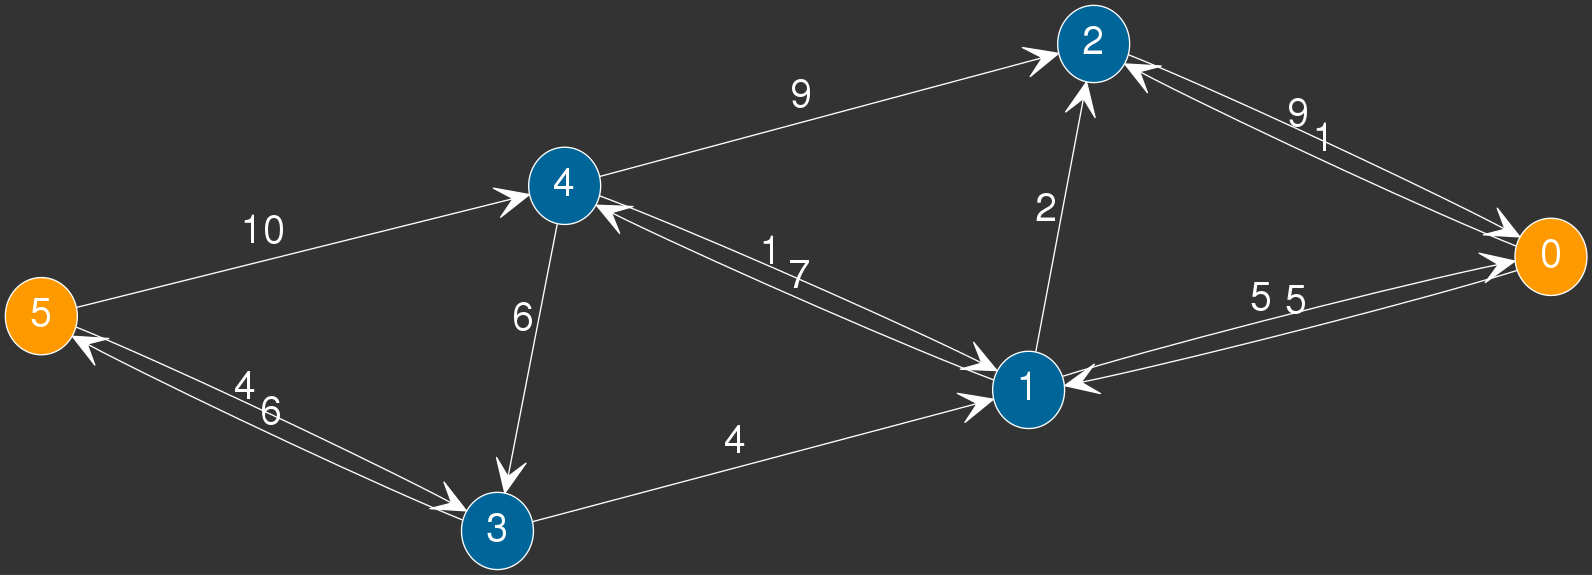
\includegraphics[width=7cm, height=4cm,center]{p5.png}
\caption{Residual Graph}
\label{fig:subim1}
\end{subfigure}
\begin{subfigure}{0.5\textwidth}
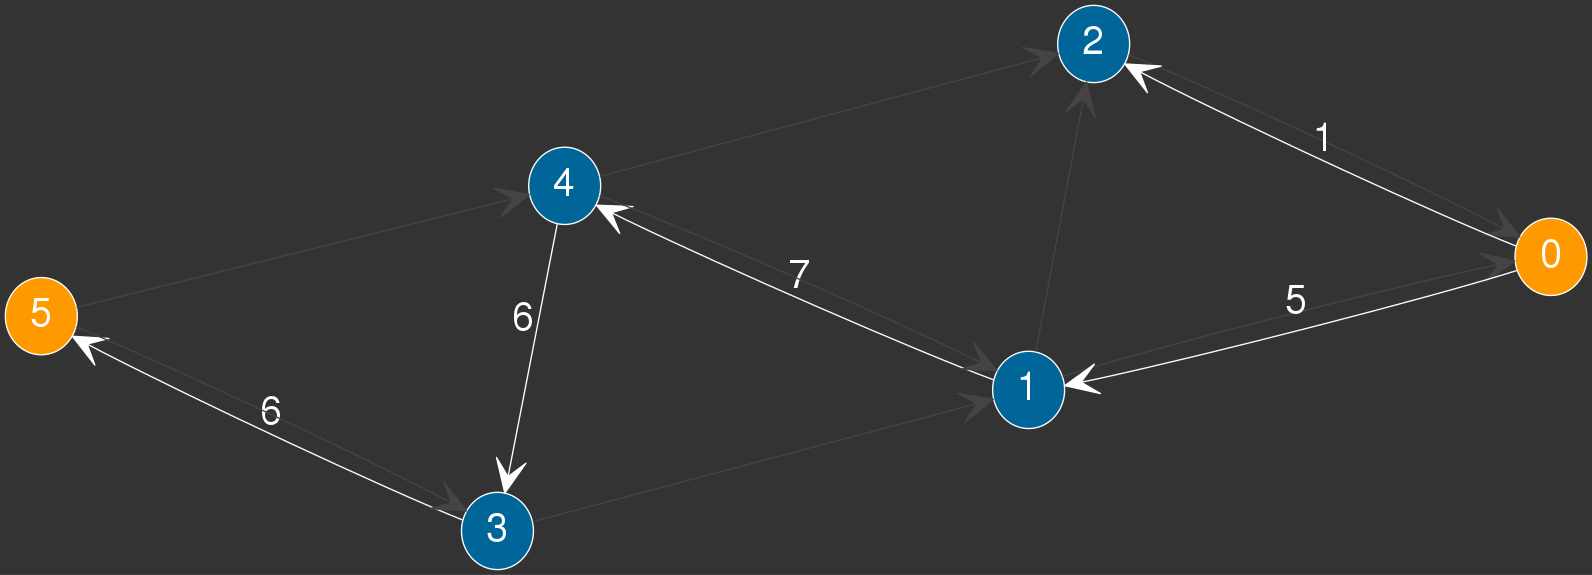
\includegraphics[width=7cm, height=4cm,center]{p7.png}
\caption{Level-graph from Residual graph}
\label{fig:subim2}
\end{subfigure}

\caption{Example for Level graph}
\label{fig:image2}
\end{figure}
%------------------------------------------------

\subsection{Augmenting path}

Given a flow-network and it's corresponding maximum capacities, an augmenting path is a source-sink path, where all the edges have the flow strictly less than the maximum capacity of the edge. Augmenting path's are used to increase the source-sink flow. If one finds an Augmenting path, then one can increase the flow along that path by Min( C\textsubscript{uv} - F\textsubscript{uv} ) for all edges E\textsubscript{uv} such that E\textsubscript{uv} belongs to the Augmenting Path. Note F\textsubscript{uv} and C\textsubscript{uv} denote the flow and capacity values. Figure \textit{2.3} highlights an augmenting path, and the flow along the path is increase by 4.

\begin{figure}[H]
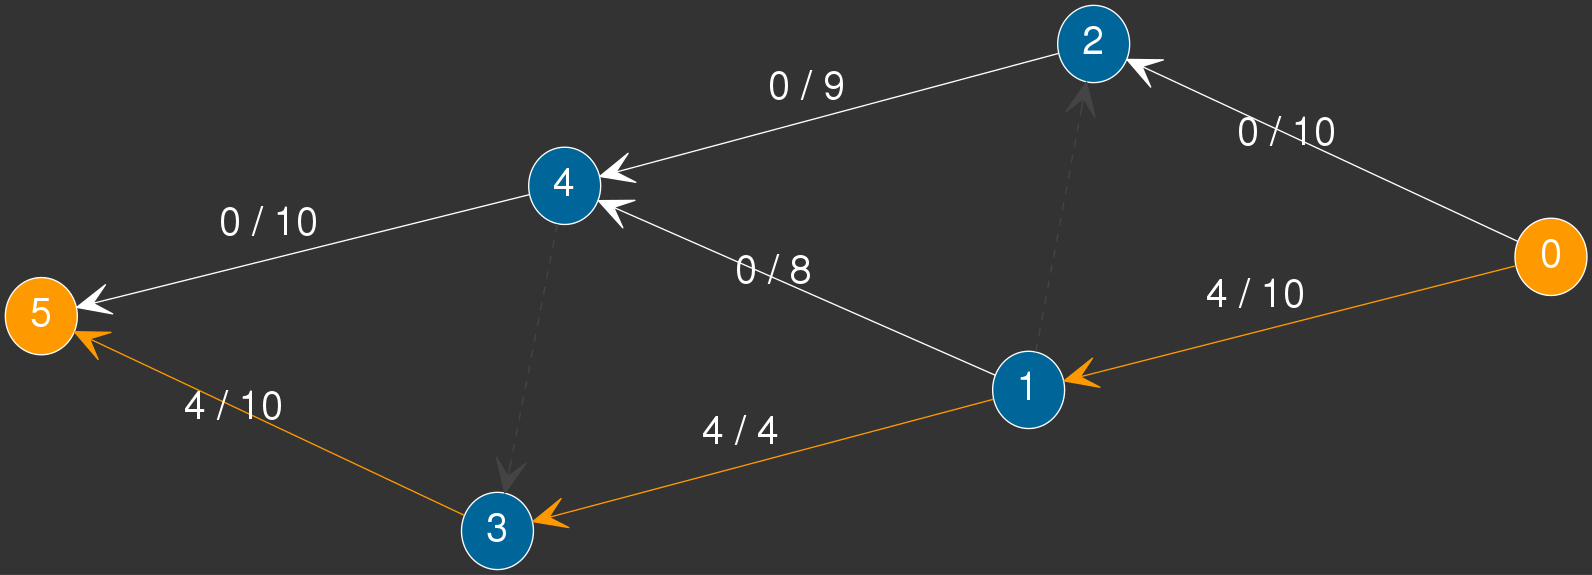
\includegraphics[width=7cm, height=4cm,center]{p8.png}
\caption{Augmenting Path denoted in Orange}
\label{fig:figure2}
\end{figure}

%----------------------------------------------------------------------------------------


\subsection{Blocking Flow}

Blocking Flow is a flow network where all possible source-sink paths have atleast one saturate edge i.e. C\textsubscript{uv} = F\textsubscript{uv} for atleast one edge E\textsubscript{uv}, along any source-sink path. Alternatively, the graph has no Augmenting Path. A blocking flow need not be a maxflow, but the converse is true.


\begin{figure}[H]
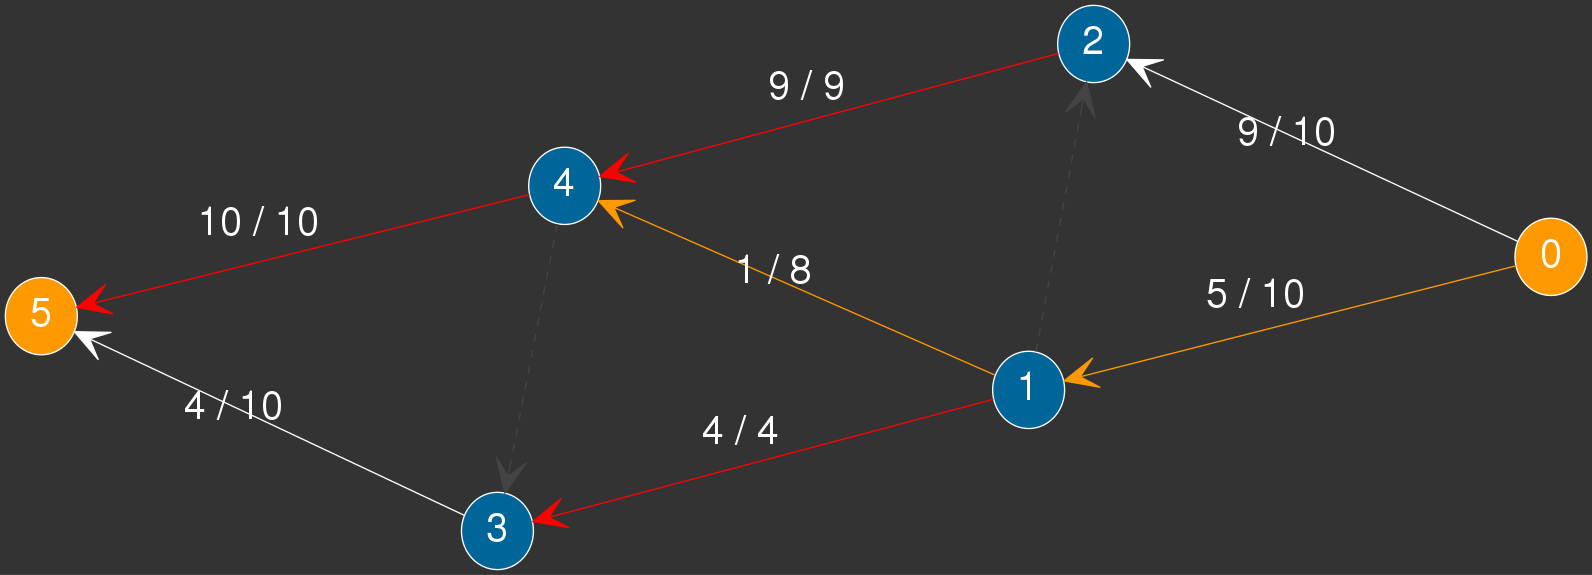
\includegraphics[width=7cm, height=4cm,center]{p9.png}
\caption{ Blocking Flow with Red, denoting that the edge is saturated}
\label{fig:figure2}
\end{figure}


%----------------------------------------------------------------------------------------


\section{Algorithm}



%----------------------------------------------------------------------------------------

\subsection{Psuedo Code}

\begin{algorithm}[H]
\KwData{Graph capacities}
\KwResult{Maxlflow network and maxflow value}
\textbf{Initialization} : Set the flow network values to be zero for all edges \;

\For{(i=1 ; i<=V ; i++)}{

G' = Level (Residual(G))\;

G' = BlockingFlow (G') 

Increment edges in G with values from G'\
}
\Return G
\caption{Dinic Algorithm}
\end{algorithm}

%----------------------------------------------------------------------------------------

As mentioned earlier, the Run-time of the algorithm is $\mathcal{O}(V^2E)$. Finding the Level graph or Residual graph takes $\mathcal{O}(E)$ since, it suffices to iterate over all edges in the graph. A blocking flow can be found in $\mathcal{O}(VE)$. Combining these two results, we get the required complexity of the algorithm.

The complexity for the blocking flow is not trivially true. The Blocking Flow routine calls the Modified DFS E times. 

\begin{align} 
\begin{split}
T(Blocking Flow) = E \times T(DFS Routine)
\end{split}					
\end{align}

Each DFS routine takes $\mathcal{O}(V)$ time to find a source-sink path in each iteration. Additionally, over all the E iterations in the Blocking Flow routine, the DFS routine can delete atmost of E edges.

Note that :

T(DFS path finding) = $\mathcal{O}(V)$

T(DFS Deletion over E function calls) = $\mathcal{O}(E)$

\begin{align} 
\begin{split}
T(Blocking Flow) = E * T(DFS path finding) + T(DFS Deletion )
\end{split}					
\end{align}


\begin{align} 
\begin{split}
\implies T(Blocking Flow) = $\mathcal{O}(VE)$
\end{split}					
\end{align}



%----------------------------------------------------------------------------------------

\begin{algorithm}[H]
\KwData{Graph capacities}
\KwResult{Blocking Flow of the Graph}
\textbf{Init} : Set the flow network values to be zero for all edges and Path\_Exists = Yes

\While{Path\_Exists=Yes}{

Path = Modified DFS(G)

\tcc{Find Augmenting Path}

\eIf{No Path found}{
   Path\_Exists = No\;
   }{
   Increase flow along Augmenting Path in G 
  }

}
\Return G
\caption{Blocking Flow}
\end{algorithm}


%----------------------------------------------------------------------------------------

\begin{algorithm}[h]
\KwData{Flow Network}
\KwResult{Augmenting Path}

Do DFS from source

Stop DFS if sink is reached

Delete Vertex is no Source-sink path possible from Vertex

\eIf{Sink encountered}{
    Augmenting\_Path = Path found from DFS 

    }{

    Augmenting\_path = None

    \tcc{If Sink, never encountered then no Source-Sink path exists}
  }

\Return Augmenting\_path
\caption{Modified DFS}
\end{algorithm}




%----------------------------------------------------------------------------------------

\subsection{Correctness}

\subsubsection{Termination}
Firstly, we shall prove that the algorithm always terminates. Each iteration in the Dinic function always, increases the source-sink distance in the level Graph. If this is true,since, the source-sink distance is less than V, termination is ensured

Using proof by contradiction, assume that the source-sink distance does not change, after updating the graph with a blocking flow. Path present in the previous iteration cannot exist in current iteration since, 

\vspace{5mm} 
\exists E\textsubscript{uv}, such that F\textsubscript{uv} = C\textsubscript{uv}, 

\vspace{5mm} 

Hence this edge will be removed in the Residual graph and hence the path cannot be present in the next iteration.
Hence new edge must be present in the path. Any new edge must be from Level 'i' to Level 'j' where 'i'>=j'. Note that the edges are with respect to the previous iteration. No edges can go to higher levels, by virtue of construction of the level graph. Hence since edges, are constrained by being from Level 'i' to Level 'j' where 'i'>=j', there can exist no source-sink path that is of same length as previous iteration. Hence we see that the algorithm terminates.


\subsubsection{Correct Result}





%----------------------------------------------------------------------------------------

\end{document}
